{
{\Large Polarization}

\definecolor{HorizontalBlue}{rgb}{.7,.7,1}
\definecolor{VerticalRed}{rgb}{1,.7,.7}

\psset{unit=0.3in}%Changes scale of plot
\psset{viewpoint=1 1 1}

%Plot axis
\newlength{\nVOffset}  \setlength{\nVOffset}{-.3in} %Vertical Offset of all axis

\newcommand{\BackAxisLabel}[1]{% Axis labels hidden behind plot
	\newcommand{\nAxisLength}{1.3}% Length of XY axis
	\ThreeDput[normal=1 0 0 ]{%Vertical label
		\textcolor{VerticalRed}{
			\psline[linecolor=VerticalRed]{-}(0,-\nAxisLength)(0,\nAxisLength)
		}
	}
	\ThreeDput[normal=0 0 1,embedangle=90]{%Horizontal label
		\textcolor{HorizontalBlue}{
			\psline[linecolor=HorizontalBlue]{-}(0,-\nAxisLength)(0,\nAxisLength)
		}
	}
	\uput{2pt}[270](0,-1.3){\textcolor{white}#1}%Plot label
}
\newcommand{\FrontAxisLabel}{% Axis labels in front of plot
	\ThreeDput[normal=1 0 0]{% Space label
		\psline[linecolor=white,linestyle=solid]{cc->}(0.55,0)(1.9,0)
	}
}

\begin{itemize}
\item%
\begin{tabular}[t]{@{}l@{\hspace{0.1in}}l}%
\begin{minipage}[t]{1.6in}EMR will travel through space linearly with no rotation, or elliptically or circularly where its axis of electrical and magnetic fluctuations are rotated. The electrical field is shown here:
 \end{minipage}&
\newlength{\nPolarityHeight}   \setlength{\nPolarityHeight}{0.8in}
%I could not figure out how to have axis lines partlty hidden by Elliptical or Circular plot
 \raisebox{0.15\nPolarityHeight}{
\begin{minipage}{2.6in}{
	\rput(0.1\linewidth,\nVOffset){%Linear polarization
		\begin{pspicture}(0,0)
		\BackAxisLabel{Linear}
		\ThreeDput[normal=1 0 0]{% Space axis
			\psline[linecolor=white,linestyle=solid]{cc->}(-.05,0)(1.6,0)
		}
		\parametricplotThreeD[xPlotpoints=200,
			linecolor=red,%
			fillstyle=none,%
			linewidth=1.5pt,plotstyle=curve,
			algebraic](0,20){0 | t/20 | sin(t)} %Formula for xyz
		\end{pspicture}
	}
	\rput(0.45\linewidth,\nVOffset){%Elliptical polarization
		\begin{pspicture}(0,0)
		\BackAxisLabel{Elliptical}
		\ThreeDput[normal=1 0 0]{% Space axes
			\psline[linecolor=white,linestyle=solid]{cc-}(-.05,0)(1.6,0)
		}
		\parametricplotThreeD[xPlotpoints=200,
			linecolor=red,%
			fillstyle=none,%
			linewidth=1.5pt,plotstyle=curve,
			algebraic](0,20){cos(t)/2 | t/20 | sin(t)} %Formula for xyz
		\FrontAxisLabel
		\end{pspicture}
	}
	\rput(0.8\linewidth,\nVOffset){%Circular polarization
		\begin{pspicture}(0,0)
		\BackAxisLabel{Circular}
		\ThreeDput[normal=1 0 0]{% Space axes
			\psline[linecolor=white,linestyle=solid]{cc-}(-.05,0)(1.6,0)
		}
		\parametricplotThreeD[%
			xPlotpoints=200,%
			hiddenLine,%
			linecolor=red,%
			fillstyle=none,%
			linewidth=1.5pt,plotstyle=curve,
			algebraic](0,20){cos(t) | t/20 | sin(t)} %Formula for xyz
	% 		\multido{\nA=0+0.1,\rA=0+5}{18}{% field strength arrows
	% 			\pstThreeDLine[linecolor=red, linewidth=1pt, arrows=->]%
	%			(0,\nA,0)(\rA\space cos \nSize\space mul,\nA,\rA\space sin \nSize\space mul)
	% 		}
		\FrontAxisLabel
		\end{pspicture}
	}
}\end{minipage}}
\end{tabular}

\vspace{0.01in}



\item Some crystals cause the photon to rotate its polarization.

\item Receivers that expect polarized photons will not accept photons that are in other polarities. (ex.\ satellite dish receivers have horizontal and vertical polarity positions).

\newlength{\nPolarizerWidth}   \setlength{\nPolarizerWidth}{0.9in}
\item
\begin{tabular}[t]{@{}l@{\hspace{0.07in}}l}
 \begin{minipage}[t]{3.25in}Polarized filters (like Polaroid\texttrademark\  sunglasses) can be used to demonstrate polarized light. One filter will only let photons that have one polarity through. Two overlapping filters at right angles will almost completely block the light that exits. The Dirac three polarizers experiment shows that a third filter inserted between the first two at \si{45\degree} allows some light to come out the end of all three filters.\end{minipage}&
 
\raisebox{-.5\nPolarizerWidth}{
	\begin{minipage}{.55in}
		{\psframebox[
			cornersize=absolute,
			linearc=4pt,
			framesep=0pt,
			fillstyle=solid,
			fillcolor=white,
			]{
			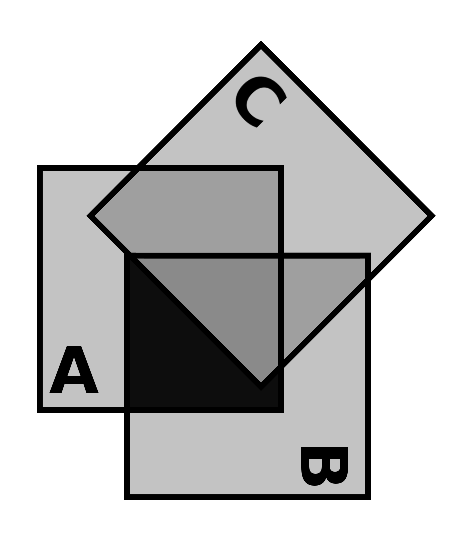
\includegraphics[width=\nPolarizerWidth]{pictures/polarizers.eps}
		}}
	\end{minipage}
}
	
\end{tabular}

% Reference: REFLECTION OF LIGHT FROM DIELECTRIC AND CONDUCTOR
%            https://lecdem.physics.umd.edu/m/m7/m7-17.html
\item Reflections from an electrical insulator are polarized. Conductive reflectors do not polarize EMR.

% from Doug Welch, and extended by internet descriptions.
\item Light from a rainbow is polarized due to the reflection inside the water droplets.

\item Moonlight is slightly polarized. Rotating a polarized sunglass lens causes the moonlight to dim and brighten slightly.

\end{itemize}

}
